\chapter{Operation}

\section{Pipeline operation}
The operation of the pipeline is shown in Figure~\ref{fig:pipeline_op}. One can see that the stages are started
every 2 clock cycles ($\tau_{c}$ is the core clock period). This is needed because the least significant bit of the next
stage result is needed. Every stage has to run $n$ (the width of the operands) times for the multiplication to be complete.

\begin{figure}[H]	
\centering
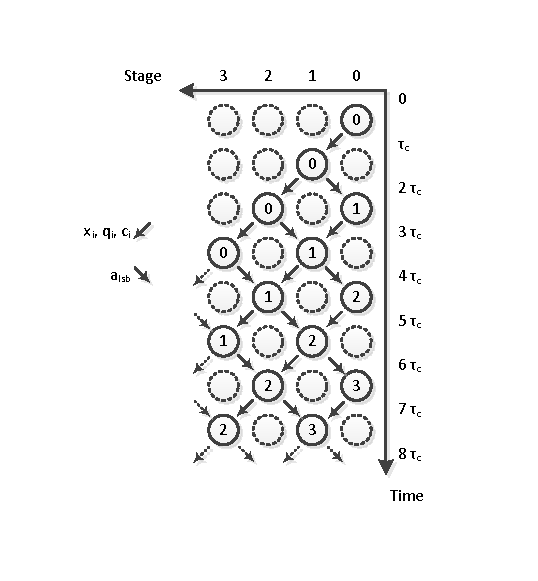
\includegraphics[trim=1.2cm 1.2cm 1.2cm 1.2cm, width=7cm]{pictures/pipeline_operation.pdf}
\caption{Pipeline operation: Each circle represents an active stage. The number indicates how much times that stage 
		has run. Dotted line contours indicate the stage is inactive.}
\label{fig:pipeline_op}
\end{figure}

For performing one Montgomery multiplication using this core, the total computation time $T_m$ for an $n$-bit operand
with a $k$-stage pipeline is given by~(\ref{eq:Tmult}).
\begin{align}\label{eq:Tmult}
T_{m} = \left[k + 2(n - 1)\right] \tau_c
\end{align}
\newpage
\section{Modular Simultaneous exponentiation operations}
Exponentiations are calculated with Algorithm~\ref{alg:mme} which uses the Montgomery multiplier as the main computation
step. It uses the principle of a square-and-multiply algorithm to calculate an exponentiation with 2 bases.
\begin{algorithm}[H] % enter the algorithm environment
\caption{Montgomery simultaneous exponentiation} % give the algorithm a caption
\label{alg:mme} % and a label for \ref{} commands later in the document
\algnewcommand\algorithmicdownto{\textbf{downto}}
\algrenewtext{For}[3]%
{\algorithmicfor\ #1 $\gets$ #2 \algorithmicdownto\ #3 \algorithmicdo}
\algnewcommand\algorithmicswitch{\textbf{switch}}
\algrenewtext{While}[2]%
{\algorithmicswitch\ #1, #2}
\algnewcommand\algorithmicinput{\textbf{Input:}}
\algnewcommand\Input{\item[\algorithmicinput]}
\algnewcommand\algorithmicoutput{\textbf{Output:}}
\algnewcommand\Output{\item[\algorithmicoutput]}
\footnotesize
\begin{algorithmic}[1] % enter the algorithmic environment
\Input $g_{0},\:g_{1},\:e_{0}=(e_{0_{t-1}} \cdots e_{0_{0}})_{2},\:e_{1}=(e_{0_{t-1}} \cdots e_{0_{0}})_{2},\:R^{2}\bmod m,\:m$
\Output $g_{0}^{e_{0}} \cdot g_{1}^{e_{1}} \bmod m$
\State $\tilde{g}_{0} := \text{Mont}(g_{0}, R^{2}),\:\tilde{g}_{1} := \text{Mont}(g_{1}, R^{2}),\:\tilde{g}_{01} := \text{Mont}(\tilde{g}_{0}, \tilde{g}_{1})$
\State $a := \text{Mont}(R^{2}, 1)$
\Comment This is the same as $a := R \bmod m$.
\For{$i$}{$(t-1)$}{0}
\State $a := \text{Mont}(a, a)$
\While{$e_{1_{i}}$}{$e_{0_{i}}$} % use as switch statement
\State $0,\:1:\;a := \text{Mont}(a, \tilde{g}_{0})$
\State $1,\:0:\;a := \text{Mont}(a, \tilde{g}_{1})$
\State $1,\:1:\;a := \text{Mont}(a, \tilde{g}_{01})$
\EndWhile
\EndFor
\State $a := \text{Mont}(a, 1)$
\State \Return{$a$}
\end{algorithmic}
\end{algorithm}
It can be seen that the algorithm requires $R^{2}\bmod m$ which is $2^{2n}\bmod m$. We assume $R^2 \bmod m$ can be
provided or pre-computed. The for loop in the algorithm is executed by the control logic of the core. Apart from this,
a few pre- and one post-calculations have to be performed.

The computation time for an exponentiation depends on the number of zero's in the exponents, from
Algorithm~\ref{alg:mme} one can see that if both exponent bits are zero at a time, no multiplication has to be
performed. Thus reducing the total time. The average computation time for a modular simultaneous exponentiation, with
$n$-bit base operands and $t$-bit exponents is given by~(\ref{eq:Tsime}).
\begin{align}\label{eq:Tsime}
T_{se} = \frac{7}{4} t \cdot T_{m} = \frac{7}{4}t \cdot [k + 2(n - 1)] \tau_c 
\end{align}

For single base exponentiations, i.e. 1 exponent is equal to zero, the average exponentiation time is given by~(\ref{eq:Texp}).
\begin{align}\label{eq:Texp}
T_{e} = \frac{3}{2} t \cdot T_{m} = \frac{3}{2}t \cdot [k + 2(n - 1)] \tau_c 
\end{align}

The formulas~(\ref{eq:Tsime}) and~(\ref{eq:Texp}) given here are only the theoretical average time for an exponentiation,
excluding the pre- and post-computations.


\section{Core operation steps}
The core can operate in 2 modes, multiplication or exponentiation mode. The steps required to do one of these actions
are described here.
\subsection{Single Montgomery multiplication}
The following steps are needed for a single Montgomery multiplication:
\begin{enumerate}
  	\item load the modulus to the RAM using the 32 bit bus
	\item load the desired $x$ and $y$ operands into any 2 locations of the operand RAM using the 32 bit bus.
	\item select the correct input operands for the multiplier using \verb|x_sel_single| and \verb|y_sel_single|
	\item select the result destination operand using \verb|result_dest_op|
	\item set \verb|exp/m| = `0' to select multiplication mode
	\item set \verb|p_sel| to choose which pipeline part you will use
	\item generate a start pulse for the core
	\item wait until interrupt is received and read out result in selected operand
\end{enumerate}

\textbf{Note:} this computation gives a result \( r = x \cdot y \cdot R^{-1} \bmod m\). If the actual product of $x$ and $y$ is
desired, a final Montgomery multiplication of the result with $R^{2}$ is needed.

\subsection{Modular simultaneous exponentiation}
The core requires $\tilde{g}_{0}$, $\tilde{g}_{0}$, $\tilde{g}_{01}$ and $a$ to be loaded into the correct operand
spaces before starting the exponentiation. These parameters are calculated using single Montgomery multiplications as follows:
\begin{align*}
	\tilde{g}_{0} &= Mont(g_{0}, R^{2}) &\,&= g_{0} \cdot R \bmod m & \hspace{3cm}\text{in operand 0}\hspace{4cm}\\
	\tilde{g}_{1} &= Mont(g_{1}, R^{2}) &\,&= g_{1} \cdot R \bmod m & \hspace{3cm}\text{in operand 1}\hspace{4cm}\\
	\tilde{g}_{01} &= Mont(\tilde{g}_{0}, \tilde{g}_{1}) &\,&= g_{0} \cdot g_{1} \cdot R \bmod m & \hspace{3cm}\text{in operand 2}\hspace{4cm}\\
	a &= Mont(R^{2}, 1) &\,&= R \bmod m &\hspace{3cm}\text{in operand 3}\hspace{4cm}
\end{align*}
When the exponentiation is done, a final multiplication has to be started by the software to multiply $a$ with 1.
The steps needed for a full simultaneous exponentiation are:


\begin{enumerate}
  	\item load the modulus to the RAM using the 32 bit bus
	\item load the desired $g_0$, $g_1$ operands and \(R^{2} \bmod m\) into the operand RAM using the 32 bit bus.
	\item set \verb|p_sel| to choose which pipeline part you will use
	\item compute $\tilde{g}_{0}$ by using a single Montgomery multiplication of $g_{0}$ with $R^{2}$ and place the result $\tilde{g}_{0}$ in operand 0.
	\item compute $\tilde{g}_{1}$ by using a single Montgomery multiplication of $g_{1}$ with $R^{2}$ and place the result $\tilde{g}_{1}$ in operand 1.
	\item compute $\tilde{g}_{01}$ by using a single Montgomery multiplication of $\tilde{g}_{0}$ with $\tilde{g}_{1}$ and place the result $\tilde{g}_{01}$ in operand 2.
	\item compute $a$ by using a single Montgomery multiplication of $R^{2}$ with $1$ and place the result $a$ in operand 3.
	\item set the core in exponentiation mode ($exp/m$='1')
	\item generate a start pulse for the core
	\item wait until interrupt is received
	\item perform the post-computation using a single Montgomery multiplication of $a$(in operand 3) with 1 and read out result
\end{enumerate}